
\begin{figure} \centering
    \begin{subfigure}{.8\textwidth}
        \begin{tikzpicture}
            \draw[->] (0, 0) node [anchor=east] {m} -- ++(1, 0) node (encrypt) [anchor=west, draw] {Encrypt};
            \path (encrypt.north) -- +(0, 0.3) pic [anchor=west, scale=0.1, red, fill=red] {key};
            \draw[->] (encrypt.east) -- ++(2, 0) node [anchor=south] {c} -- ++(2,0) node (decrypt) [anchor=west, draw] {Decrypt};
            \path (decrypt.north) -- +(0, 0.3) pic [anchor=west, scale=0.1, red, fill=red] {key};
            \draw[->] (decrypt.east) -- ++(1,0) node [anchor=west] {m'};
        \end{tikzpicture}
        \caption{Symmetric Encryption: Both keys are identical.} \label{fig:keys-symmetric}
    \end{subfigure}
    \\
    \vspace{0.5cm}
    \begin{subfigure}{.8\textwidth}
        \begin{tikzpicture}
            \draw[->] (0, 0) node [anchor=east] {m} -- ++(1, 0) node (encrypt) [anchor=west, draw] {Encrypt};
            \path (encrypt.north) -- +(0, 0.3) pic [anchor=west, scale=0.1, olive, fill=olive] {key};
            \draw[->] (encrypt.east) -- ++(2, 0) node [anchor=south] {c} -- ++(2,0) node (decrypt) [anchor=west, draw] {Decrypt};
            \path (decrypt.north) -- +(0, 0.3) pic [anchor=west, scale=0.1, red, fill=red] {key};
            \draw[->] (decrypt.east) -- ++(1,0) node [anchor=west] {m'};
        \end{tikzpicture}
        \caption{Asymmetric Encryption: Different keys for encryption and decryption. Decryption succeeds if and only if the decryption key is exactly the counterpart to the encryption key.} \label{fig:keys-asymmetric}
    \end{subfigure}
    \\ 
    \vspace{0.5cm}
    \begin{subfigure}{.8\textwidth}
        \begin{tikzpicture}[sibling distance=4mm, level distance=3mm]
            \draw[->] (0, 0) node [anchor=east] {m} -- ++(1, 0) node (encrypt) [anchor=west, draw] {Encrypt};
            
            \scoped{
                \tikzstyle{every node}=[fill, circle, draw, inner sep=0.5mm];
                \tikzstyle{level 2}=[sibling distance=1.5mm];
                \fill[red] (decrypt.north) -- ++(0, 0.7) node [anchor=south] {} child {node {} child {node {}} child {node {}} child {node {}}} child { node {} child {node {}}};
            };
            \draw[->] (encrypt.east) -- ++(2, 0) node [anchor=south] {c} -- ++(2,0) node (decrypt) [anchor=west, draw] {Decrypt};
            \path (encrypt.north) -- +(0, 0.3) node [olive] {$\{A, B, C\}$};
            \draw[->] (decrypt.east) -- ++(1,0) node [anchor=west] {m'};
        \end{tikzpicture}
        \caption{\glslink{gls-kp-abe}{Key-Policy Attribute-Based Encryption}: Attributes for encryption, access structure for decryption. Decryption succeeds if and only if the attributes of the ciphertext satisfy the policy embedded in the key.} \label{fig:keys-abe}
    \end{subfigure}
    \\ 
    \vspace{0.5cm}
    \begin{subfigure}{.8\textwidth}
        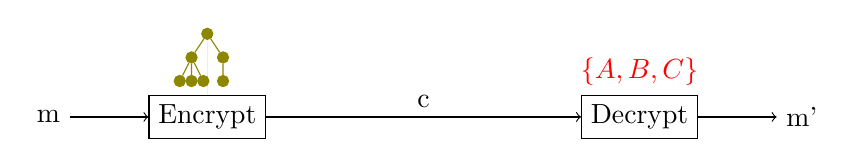
\begin{tikzpicture}[sibling distance=4mm, level distance=3mm]
            \draw[->] (0, 0) node [anchor=east] {m} -- ++(1, 0) node (encrypt) [anchor=west, draw] {Encrypt};
            
            \scoped{
                \tikzstyle{every node}=[fill, circle, draw, inner sep=0.5mm];
                \tikzstyle{level 2}=[sibling distance=1.5mm];
                \fill[olive] (encrypt.north) -- ++(0, 0.7) node [anchor=south] {} child {node {} child {node {}} child {node {}} child {node {}}} child { node {} child {node {}}};
            };
            \draw[->] (encrypt.east) -- ++(2, 0) node [anchor=south] {c} -- ++(2,0) node (decrypt) [anchor=west, draw] {Decrypt};
            \path (decrypt.north) -- +(0, 0.3) node [red] {$\{A, B, C\}$};
            \draw[->] (decrypt.east) -- ++(1,0) node [anchor=west] {m'};
        \end{tikzpicture}
        \caption{\glslink{gls-cp-abe}{Ciphertex-Policy Attribute-Based Encryption}: \Gls{access-policy} for encryption, attributes for decryption. Decryption succeeds if and only if the attributes of the key match the policy embedded in the ciphertext.} \label{fig:keys-abe}
    \end{subfigure}
    \caption[Keys in different classes of encryption schemes]{Keys used for encryption and decryption in different classes of encryption schemes. Red information has to be kept secret, green information may be made publicly available. For the differences between the two types of \acrshort{abe}, see Section~\ref{sec:cp-vs-kp}.}
    \label{fig:key-use}
\end{figure}